\RequirePackage[l2tabu, orthodox]{nag}
\documentclass[12pt]{article}
\usepackage[utf8]{inputenc}
\usepackage[spanish,es-lcroman, es-tabla]{babel}
\usepackage[autostyle,spanish=mexican]{csquotes}
\usepackage{amsmath}
\usepackage{amssymb}
\usepackage{nccmath}
\numberwithin{equation}{section}
\usepackage{amsthm}
\usepackage{graphicx}
\usepackage{epstopdf}
\DeclareGraphicsExtensions{.pdf,.png,.jpg,.eps}
\usepackage{color}
\usepackage{float}
\usepackage{multicol}
\usepackage{enumerate}
\usepackage[shortlabels]{enumitem}
\usepackage{anyfontsize}
\usepackage{anysize}
\usepackage{array}
\usepackage{multirow}
\usepackage{enumitem}
\usepackage{cancel}
\usepackage{tikz}
\usepackage{circuitikz}
\usepackage{tikz-3dplot}
\usetikzlibrary{babel}
\usetikzlibrary{shapes}
\usepackage{bm}
\usepackage{mathtools}
\usepackage{esvect}
\usepackage{hyperref}
\usepackage{relsize}
\usepackage{siunitx}
\usepackage{physics}
%\usepackage{biblatex}
\usepackage{standalone}
\usepackage{mathrsfs}
\usepackage{bigints}
\usepackage{bookmark}
\spanishdecimal{.}

\setlist[enumerate]{itemsep=0mm}

\renewcommand{\baselinestretch}{1.5}

\let\oldbibliography\thebibliography

\renewcommand{\thebibliography}[1]{\oldbibliography{#1}

\setlength{\itemsep}{0pt}}
%\marginsize{1.5cm}{1.5cm}{2cm}{2cm}


\newtheorem{defi}{{\it Definición}}[section]
\newtheorem{teo}{{\it Teorema}}[section]
\newtheorem{ejemplo}{{\it Ejemplo}}[section]
\newtheorem{propiedad}{{\it Propiedad}}[section]
\newtheorem{lema}{{\it Lema}}[section]

\pagestyle{fancy}
\fancyhf{}
\rhead{Examen - Tarea 3}
\rfoot{\thepage}
\renewcommand{\headrulewidth}{0.5pt}
\setlength{\headheight}{30pt} 
%\usepackage[left=1.5cm,top=1.5cm,right=1.5cm,bottom=1.5cm]{geometry}
\title{Examen Tarea 3 - Funciones especiales \\ \large{Matemáticas Avanzadas de la Física}}
\date{ }
\begin{document}
\vspace{-4cm}
\maketitle
\fontsize{14}{14}\selectfont
\begin{enumerate}
\item Una esfera conductora de calor de radio $a$ está compuesta por dos hemisferios con un espacio infinitesimal aislante entre ellos, revisa la figura (\ref{fig:figura2}). Las mitades superior e inferior de la esfera están en contacto con baños térmicos de temperaturas $+ T_{1}$ y $-T_{1}$, respectivamente. La esfera está dentro de otra esfera conductora de calor de radio $b$ con una temperatura $T_{2}$. Encuentra la temperatura en los puntos:
\begin{enumerate}[label=\alph*)]
\item Dentro de la esfera interior,
\item En la región entre las dos esferas y
\item Por fuera de la esfera exterior.
\end{enumerate} 
\begin{figure}[!ht]
\centering
\includestandalone{Figuras/esfera1}
\caption{La esfera interior se encuentra a diferente temperatura.}
\label{fig:figura2}
\end{figure}
\item Considera una esfera conductora neutra radio $a$ dentro un campo eléctrico uniforme  $E_{0}$ que suponemos es de extensión infinita, como se muestra en la figura (\ref{fig:figura3}). Queremos encontrar el potencial electrostático en cualquier punto fuera de la esfera. Justifica cada uno de los pasos que decidas utilizar para resolver el problema.
\begin{figure}[!ht]
\centering
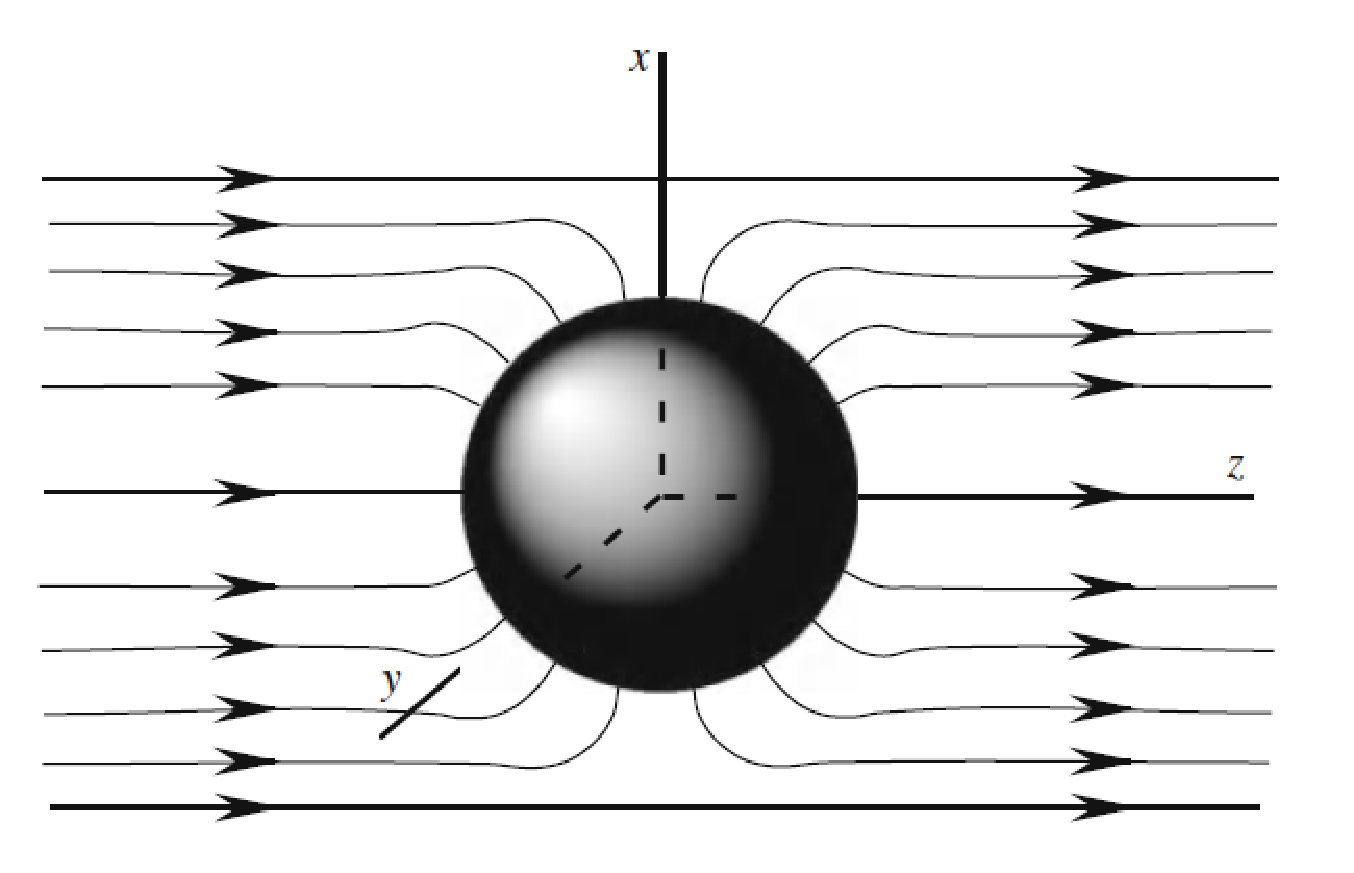
\includegraphics[scale=0.5]{Imagenes/Esfera_Tarea5.eps}
\caption{Esfera conductora neutra inmersa en un campo eléctrico uniforme.}
\label{fig:figura3}
\end{figure}
\item Un cilindro largo conductor de calor de radio $a$ se compone de dos mitades (con secciones transversales semicirculares) con un espacio infinitesimal entre ellas. Las mitades superior e inferior del cilindro están en contacto con baños térmicos $+T_{0}$ y $-T_{0}$, respectivamente. Encuentra la temperatura tanto dentro como fuera del cilindro.
\item Un cilindro largo conductor de calor de radio $a$ se compone de dos mitades (con secciones transversales semicirculares) con un espacio infinitesimal entre ellas. Las mitades superior e inferior del cilindro están en contacto con baños térmicos $+T_{1}$ y $-T_{1}$, respectivamente. El cilindro está dentro de otro cilindro de radio  $b$ más grande ( $a < b$ y coaxial con él) que se mantiene a la temperatura $T_{2}$. Encuentra la temperatura dentro del cilindro interno, entre los dos cilindros y fuera del cilindro externo.
\item La transición de probabilidad entre dos estados $\psi_{m}$ y $\psi_{n}$ del oscilador armónico cuántico, depende de que el valor de la siguiente integral sea:
\[ \int_{-\infty}^{\infty} x \; e^{-x^{2}} \; H_{n} (x) \, H_{m}(x) \dd x = \sqrt{\pi} \; 2^{n-1} \; n! \; \delta_{m,n+1} + \sqrt{\pi} \; 2^{n} \; (n+1)! \; \delta_{m,n+1} \]
Obtén explícitamente este valor. El resultado muestra que las transiciones sólo pueden ocurrir entre estados cuyos niveles de energía sean adyacentes, $m = n \pm 1$
% \item Deducir una expresión para la distribución estacionaria de temperaturas $u(r,z)$ en un cilindro macizo limitado por las superficies $r = 1$, $z = 0$ y $z = 1$, si $u = 0$ en la superficie $r = 1$, $u = 1$ en la superficie $z = 1$ y la base $z = 0$ está aislada.
\item Desarrollar el potencial electrostático en términos de polinomios de Legendre, de un arreglo de cargas como se muestra en la figura (\ref{fig:figura1}), que representa un cuadropolo eléctrico.
\begin{figure}[H]
\centering
\includestandalone{Figuras/cuadrupolo}
\caption{Cuadropolo eléctrico.}
\label{fig:figura1}
\end{figure}
\item Obtener la expasión de la función delta de Dirac en términos de los polinomios de Legendre.
\item El estado normal del átomo de hidrógeno es el de más baja energía, $(n = 1)$. Le corresponde una función de onda:
\[ \psi_{100} = \dfrac{1}{\sqrt{\pi \, a_{0}^{3}}} \, e^{-r/a_{0}}\]
donde $a_{0} = 2 \, \alpha = 4 \, \hbar^{2} \, \pi \varepsilon_{0}/ m \,q^{2}$ es el radio de Bohr. La densidad volumétrica de probabilidad de localización del electrón es $dv{P}{V} = \psi_{100}^{*} \, \psi_{100}$, de modo que $\dv{P}{r} = 4 \, \pi r^{2} \abs{\psi_{100}}^{2}$. Demuestra que la distancia más probable a la que se encuentra el electrón del núcleo es $r = a_{0}$, coincidente con el radio de la primera órbita de Bohr.
% \item Un cilindro conductor largo de radio $a$ está a un potencial $V_{1}$, éste cilindro está dentro de otro cilindro radio $b$ (comparten un eje coaxial y $a < b$) que se mantiene a un potencial $V_{2}$. Calcula el potencial dentro del cilindro de radio $a$, el potencial entre los dos cilindros y el potencial por fuera del cilindro de radio $b$.
\item \begin{enumerate}[label=\alph{*})]
\item Verifica el operador identidad
\[ x - \dv{x} = \exp(\dfrac{x^{2}}{2}) \; \dv{x} \exp \left(- \dfrac{x^{2}}{2} \right) \]
\item La función de onda normalizada del oscilador armónico es
\[ \psi_{n} (x) = \dfrac{1}{(\pi^{1/2} \; 2^{n} \; n!)^{1/2}} \; \exp \left(- \dfrac{x^{2}}{2} \right) \; H_{n}(x) \]
Demostrar que puede escribirse como
\[ \psi_{n} (x) = \dfrac{1}{(\pi^{1/2} \; 2^{n} \; n!)^{1/2}} \; \left( x - \dv{x} \right)^{n} \; \exp \left(- \dfrac{x^{2}}{2} \right) \]
\end{enumerate}
\item Los operadores de creación y aniquilamiento generan nuevas soluciones de la ecuación de Schrödinger, pero esas soluciones no están debidamente normalizadas. Por tanto $a_{+} \, \psi_{n}$ es proporcional a $\psi_{n+1}$ y $a_{-} \, \psi_{n}$ es proporcional a $\psi_{n-1}$, por lo que nos gustaría conocer las constantes de proporcionalidad. Usando integración por partes y la ecuación de Schrödinger
\begin{align*}
(a_{-} \, a_{+} - \dfrac{1}{2} \, \hbar \, \omega) \, \psi &= E \, \psi \\
(a_{+} \, a_{-} - \dfrac{1}{2} \, \hbar \, \omega) \, \psi &= E \, \psi 
\end{align*}
demostrar que
\[ \int_{-\infty}^{\infty} \abs{a_{+} \, \psi_{n}}^{2} \, \dd x = (n+1) \, \hbar \, \omega, \hspace{1.5cm} \int_{-\infty}^{\infty} \abs{a_{-} \, \psi_{n}}^{2} \, \dd x = n \, \hbar \, \omega \]
y entonces (con $i$ para que las funciones de onda sean reales)
\begin{align*}
a_{+} \, \psi_{n} &= i \, \sqrt{(n+1) \, \hbar \, \omega} \; \psi_{n+1} \\
a_{-} \, \psi_{n} &= -i \, \sqrt{n \, \hbar \, \omega} \; \psi_{n-1}
\end{align*}
\item Un análisis de la mecánica cuántica del efecto Stark (en coordenadas parabólicas) nos conduce a la ecuación diferencial
\[  \dv{\xi} \left( \xi \, \dv{u}{\xi} \right) + \left( \dfrac{1}{2} \, E \, \xi + L - \dfrac{m^{2}}{4 \, \xi} - \dfrac{1}{4} \, F \, \xi^{2} \right) u = 0 \]
Donde $F$ es una medida de la energía que perturba al sistema debida a un campo eléctrico externo. Encuentra las funciones de onda sin perturbaciones $(F=0)$ en términos de los polinomios asociados de Laguerre.
\\
Tip: a lo que tienes que llegar es a un resultado del tipo
\[ u(\xi) = \exp(- \varepsilon \, \xi /2) \; \xi^{m/2} \; L_{p}^{m} (\varepsilon \, \xi)  \]
donde $\varepsilon = \sqrt{-E} > = 0$ y $p = \alpha / \varepsilon - (m+1) / 2$ que es un entero no negativo.
\item Demostrar que $F \left(m, -m, \dfrac{1}{2}; \dfrac{(1-x)}{2} \right) = T_{m}(x)$.
\end{enumerate}
%
%\begin{thebibliography}{a}
%\bibitem{Griffiths} \textsc{Griffiths, David J.},
%\textit{Introduction to Quantum Mechanics.}
%Prentice Hall, 1995.  
%\end{thebibliography}
\end{document}